\section{Trasporto}
Il layer di rete si occupa di portare i dati da un host ad un altro host, ma il nostro scopo è trasportare dati da un processo ad un altro processo.

Il goal principale del layer trasporto è quindi il multiplexing/demultiplexing del flusso dei dati da e verso i vari processi.
Inoltre possiamo anche costruire meccanismi di trasferimento dati affidabile, controllo del flusso e controllo della congestione.

Abbiamo principalmente due protocolli TCP e UDP.

\subsection{Multiplexing \& Demultiplexing}
Il demultiplexing consiste nello smistamento del traffico in arrivo verso un host nei singoli processi che l' host ospita.
Questo può essere ottenuto tramite l' utilizzo del numero di porta, ogni processo che ha intenzione di comunicare tramite la rete è in ascolto su una porta, quando l' host riceve del traffico indirizzato su quella porta provvede ad inoltrarlo al singolo processo.

\subsubsection{Demultiplexing su servizio datagramma}
L' host riceve datagrammi IP, ogni datagramma contiene IP sorgente e destinatario, ogni datagramma trasporta un segmento del layer trasporto ed ogni segmento contiene la porta sorgente e la porta destinataria.

\subsubsection{Demultiplexing su servizio stream}
Il socket non è più qualcosa di indipendente, un singolo socket su un host è collegato al socket sull' altra macchina, quindi si crea una vera e propria connessione.
Questa connessione è identificata da IP e porta sorgente, IP e porta desinataria.
Durante la consegna si guardano quindi tutti questi parametri.
\begin{figure}[H]
    \centering
    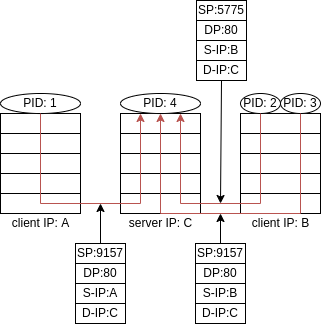
\includegraphics[width=250px]{images/6_Trasporto/demux_with_multiprocess.png}
\end{figure}
Su una porta può essere in ascolto solo un processo, tuttavia se il processo forka, i figli ereditano tutti la stessa porta e quindi in questo caso si rende molto più importante il riconoscimento della informazione tramite questi 4 parametri.

\subsection{UDP}
E' uno dei primi protocolli standardizzati nella Internet moderna.
E' un servizio di tipo best-effort quindi possiamo perdere pacchetti o vederli consegnati fuori ordine.
Di fatto è assolutamente uguale a IP ma aggiunge il multiplexing ed il demultiplexing.

\subsubsection{Perché usarlo?}
Può tornare utile per il suo essere connectionless, essendo tale non c'è necessità di aprire una connessione quindi niente overhead.
E' estremamente semplice in quanto non mantiene uno stato né nella sorgente né nella destinazione.
Ci permette di avere più controllo sui dati in quanto non abbiamo controlli di flusso o di congestione.

E' largamente utilizzato per applicazioni loss tolerant o rate sensitive come lo streaming, ma anche in altri protocolli come DNS, NFS, SNMP ed il RIP (un protocollo di routing).

\subsubsection{Formato del segmento}
\begin{figure}[H]
    \centering
    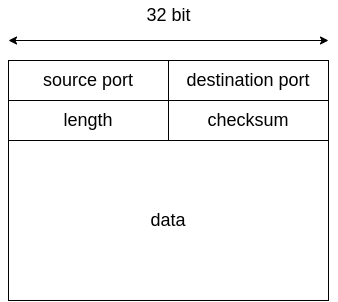
\includegraphics[width=200px]{images/6_Trasporto/udp_segment.png}
\end{figure}

\begin{itemize}
    \item porta sorgente
    \item porta di destinazione
    \item lunghezza dei dati: lunghezza del segmento UDP inclusi gli header. Misurato in byte
    \item checksum
    \item dati
\end{itemize}
La checksum è utilizzata per eseguire una error detection, è eseguito tramite somma del contenuto in blocchi da 16 bit, se c'è un carry si somma al risultato, infine si fa il complemento ad 1.


\subsection{TCP}
Offre un servizio orientato alla connessione, quindi prima di trasmettere i dati c'è necessità di aprire una connessione, si usa il cosiddetto \emph{three-way handshake}.
Questa connessione è simile alla creazione del circuito virtuale, tuttavia i dispositivi del core non lo sanno, è qualcosa che riguarda solo gli host alle estremità del circuito.

Essendo un protocollo a flusso il pacchetto viene chiamato \emph{segmento}.
Implementa una connessione punto-punto quindi con un solo trasmettitore ed un solo ricevitore.
Questa connessione è full-duplex quindi entrambi gli endpoint possono inviare e ricevere allo stesso tempo.

Grazie a questo concetto di connessione possiamo costruire una trasmissione affidabile ed in ordine, si usano quindi dei buffer per inviare e ricevere.
Implementa un controllo del flusso quindi se il trasmettitore è troppo veloce il ricevitore glielo fa sapere ed il trasmettitore abbassa il suo rateo, questo si fa guardando la dimensione del buffer di ricezione e trasmettendolo al trasmettitore.

Invia i pacchetti in pipeline implementando un controllo di flusso e di congestione basato su finestra.

\subsubsection{Formato del segmento}
\begin{figure}[H]
    \centering
    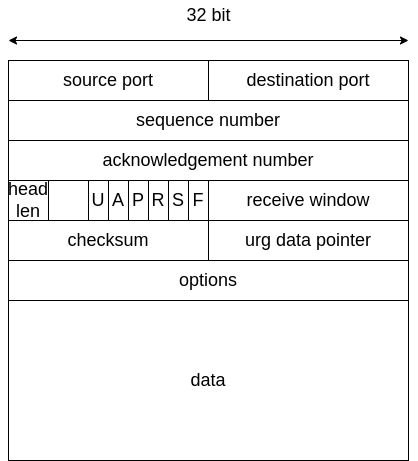
\includegraphics[width=200px]{images/6_Trasporto/tcp_segment.png}
\end{figure}

\begin{itemize}
    \item porta sorgente
    \item porta destinataria
    \item numero di sequenza: usato per dare un ordine ai segmenti inviati, parte del meccanismo di in-order delivery.
    E' orientato al byte quindi al suo interno c'è la posizione nello stream del primo byte contenuto nel segmento
    \item numero di acknowledge: valido quando il bit di ACK è attivo, indica il numero di sequenza del prossimo pacchetto che si aspetta di ricevere
    \item head len
    \item NC
    \item flags:
    \begin{itemize}
        \item URG flag: poco usato
        \item ACK flag: indica che questo segmento è un acknowledge e quindi il campo di acknowledgement number è valido
        \item PSH flag: poco usato
        \item RST, SYN, FIN: usati per la connessione e la disconnessione.
    \end{itemize}
    \item receive window: il ricevitore vi scrive lo spazio libero nel proprio buffer di ricezione
    \item checksum
    \item urg data pointer: significativo solo se il flag URG è attivo, in genere poco usato
    \item opzioni: altre informazioni generalmente poco utilizzate
    \item payload
\end{itemize}

\subsubsection{Sequence number ed ACK}
\begin{figure}[H]
    \centering
    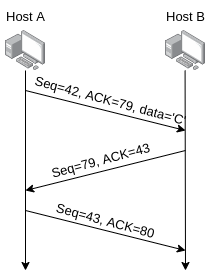
\includegraphics[width=150px]{images/6_Trasporto/sequence_number_ack.png}
\end{figure}
Il sequece number è il numero della posizione del primo byte del segmento dati nello stream.
L' ACK è il numero di sequenza del prossimo segmento che l' host si aspetta di ricevere.

L' inoltro out-of-order è gestito in maniera differente in base alle implementazioni, non c'è uno standard.

\subsubsection{Allocazione della connessione}
La fase di creazione della connessione è la fase in cui vengono allocate tutte le strutture dati necessarie per la gestione di questo meccanismo.
Da parte del client avviene quando si usa la primitiva connect(...) su un socket TCP (SOCK\_STREAM su AF\_INET).
Da parte del server avviene quando si usa la primitiva accept(...) su un socket TCP.

\subsubsection{Three-way handshake}
\begin{figure}[H]
    \centering
    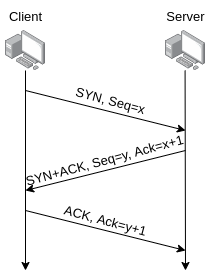
\includegraphics[width=150px]{images/6_Trasporto/threeway_handshake.png}
\end{figure}

\begin{itemize}
    \item il client invia un segmento con il flag SYN attivo, senza dati e con un sequence number iniziale generato casualmente

    \item il server riceve il segmento con il flag SYN attivo e risponde con un segmento con SYN ed ACK attivo.
    Inserisce nessun dato e specifica un sequence number generato casualmente, mentre inserisce come acknowledge number il valore del sequence ricevuto incrementato di 1.
    In questa fase il server alloca i buffer.

    \item il client riceve il segmento con SYN-ACK  e risponde con un segmento con solo ACK attivo.
    Inoltre inserisce anche l'acknowledge number come segment number ricevuto incrementato di 1.
    A questo punto potrebbe già inviare dei dati.
\end{itemize}
Si creano dei sequence number casuali per evitare che il client si connetta, chiuda subito la connessione, poi la riapra subito dopo ed allora nei buffer interni vi rimangano ancora i dati vecchi.

\subsubsection{Connection tear-down}
\begin{figure}[H]
    \centering
    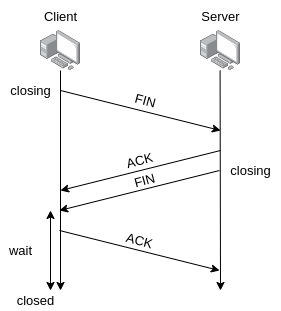
\includegraphics[width=200px]{images/6_Trasporto/connection_teardown.png}
\end{figure}

\begin{itemize}
    \item il client invia un pacchetto con il flag FIN attivo
    \item Il server lo riceve e risponde con un segmento con il flag ACK attivo, invia i dati che deve ancora inviare, chiude la connessione ed infine invia un pacchetto con FIN.
    \item il client una volta ricevuto il pacchetto di FIN risponde con un pacchetto ACK.
    Durante questo tempo il server rimane ancora in attesa di ricevere l' ACK
\end{itemize}
Se l' ACK del FIN del server non arriva o il FIN del server si perde (che sono la stessa cosa) il server provvede a re-inviare nuovamente il FIN.
Quindi sia il client che il server rimangono in attesa di avere questa conferma della chiusura della connessione.

\subsubsection{Reliable data transfer}
Il TCP crea un servizio di trasmissione affidabile usando il canale costruito da IP.
Sfrutta uno schema di tipo ARQ: Acknowledgements, Retransmissions and Timeouts basato su finestra.

L' intervallo di timeout è qualcosa che non è possibile calcolare perché dipende fortemente dal ritardo di accodamento, questo ritardo tuttavia si verifica su ogni router che si incontra quindi è casuale.
Conviene fare una stima basata sul RTT degli ultimi pacchetti inviati e la ricezione dei loro ACK.
Il primo segmento lo inviamo con un intervallo di timeout abbastanza grande e fisso, i successivi intervalli invece li calcoliamo tramite una media esponenziale mobile:
$$ ERTT_1 = RTT_0 $$
$$ ERTT_2 = \alpha \cdot RTT_1 + (1-\alpha) \cdot RTT_0 $$
$$ ERTT_3 = \alpha \cdot RTT_2 + \alpha(1-\alpha) \cdot RTT_1 + (1 - \alpha)^2 \cdot RTT_0 $$
$$ ERTT_{n+1} = \alpha \cdot RTT_n + (1 - \alpha) \cdot ERTT_n $$

\begin{itemize}
    \item RTT: round trip time misurato
    \item ERTT: estimated round trip time. $0 < \alpha < 1$
\end{itemize}

NB: $\alpha \approx 0$: da molto peso alla storia passata e poco a quella recente.

$\alpha \approx 1$: da molto peso alla storia recente e poco a quella passata.
Dopo numerose simulazioni sul campo si misura che il valore ottimale è $\alpha = 0.125$.

Ora abbiamo il valore stimato di RTT, dobbiamo trasformarlo in un intervallo di tempo da aspettare, possiamo fare diverse scelte:
\begin{itemize}
    \item secondo l' algoritmo di Karn-Partridge dovremmo usare come intervallo di tempo $2 \cdot ERTT$.
    In questo caso i pacchetti che sono stati ritrasmessi perché persi non vengono aggiunti alla stima di ERTT.
    
    \item secondo l' algoritmo di Van Jacobson - Karel si usa la stima di ERTT con aggiunta di un margine di sicurezza calcolato come: $DevRTT_{n+1} = (1-\beta)\cdot DevRTT_n + \beta\cdot|RTT_n - ERTT_n|$.
    Infine l' intervallo lo si fa di dimensione $ERTT + 4 \cdot DevRTT$.
    Tipicamente $\beta=0.25$
\end{itemize}

\subsubsection{TCP semplificato}
Vediamo come funziona una versione del TCP che ignora gli ACK duplicati, la gestione del flusso e della congestione.

Il trasmettitore come eventi può:
\begin{itemize}
    \item ricevere dati dall' applicazione: in questo caso bisogna creare un segmento con il numero di sequenza opportuno, una volta inviato bisogna far partire il timer (che è riferito sempre al pacchetto più vecchio, quindi parte se già non ce n'è uno attivo, altrimenti non ne parte uno nuovo)
    
    \item segnalazione del timeout: in questo caso si ritrasmettono i segmenti che hanno causato il timeout e si fa ripartire il timer
    
    \item ricezione di un ACK: in questo caso se l'ACK è di pacchetti non precedentemente confermati si aggiorna l' elenco dei pacchetti non confermati e si sposta il timer in modo da far riferimento al primo pacchetto non confermato.
\end{itemize}

\begin{verbatim}
// Sender
NextSeqNum = InitialSeqNum
SendBase = InitialSeqNum

while(1){
    switch event {
    case DATA_RCVD:
        packet = make_segment(NextSeqNum, data)
        if !timer:
            timer.start()
        send_data_to_network(packet)
        NextSeqNum += length(data)
    break;
    
    case TIMEOUT:
        for p in window:
            send_data_to_network(p)
        timer.start()
    break;
    
    case ACK:
        if y > SendBase:
            SendBase = y
            if NextSeqNum != SendBase:
                timer.start()
    break;
    }
}    
\end{verbatim}

Scenari di ritrasmissione:
\begin{itemize}
    \item ci perdiamo l'ACK, aspettiamo il timeout e reinviamo il segmento

    \item inseriamo il timeout troppo presto quindi ritrasmettiamo i segmenti e poco dopo ci arriva l' ACK precedente, in questo caso avremo degli ACK duplicati

    \item se inviamo più segmenti, ci perdiamo l' ACK del primo ma riceviamo quelli successivi possiamo leggerlo come ACK cumulativo e quindi non ritrasmettiamo perché diamo per scontato che il ricevitore abbia ricevuto anche quelli precedenti e che abbiamo perso l' ACK
\end{itemize}
Ogni volta che eseguiamo una ritrasmissione raddoppiamo l' intervallo di timeout (exponential increase), è una tecnica di controllo della congestione.

\subsubsection{Fast retransmission}
Il periodo di timeout spesso è troppo lungo da aspettare quindi potrebbe succedere di dover aspettare la scadenza del timer pur sapendo che alcuni pacchetti sono stati persi.
Questo può succedere quando si ricevono ACK duplicati, aggiungiamo quindi la politica che se riceviamo 3 ACK duplicati (cioè 4 ACK per lo stesso segmento) procediamo a ritrasmettere senza aspettare che il timeout scada.
\begin{figure}[H]
    \centering
    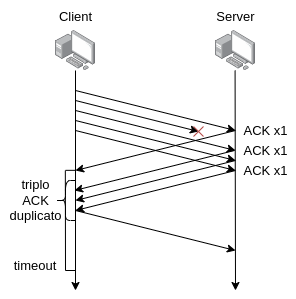
\includegraphics[width=200px]{images/6_Trasporto/fast_retransmit.png}
\end{figure}

NB: Il protocollo TCP non è propriamente né Go-Back-N né Selective Repeat, è un ibrido in quanto ritrasmette dal primo segmento non ACK (quindi non N segmenti indietro) ma non prevede l'ACKnowledge dei singoli segmenti.

\subsubsection{Sommario degli eventi}
Gli eventi del ricevitore sono quindi:
\begin{itemize}
    \item arrivo di un segmento in ordine con numero di segmento aspettato, con tutti i segmenti fino a quel punto ACKati.
    Si aspettano 500ms prima di inviare l'ACK per vedere se è in arrivo qualche altro segmento in modo da eseguire un ACK cumulativo, se non arriva si procede ad inviare l' ACK.

    \item arrivo di un segmento in ordine con un numero di segmento aspettato ma con almeno un altro segmento non ACKato.
    Si invia immediatamente un ACK cumulativo in modo da confermare tutti e due i segmenti.

    \item arrivo di un segmento out-of-order con numero di segmento più grande di quello aspettato, si ha un gap.
    Si invia immediatamente un ACK duplicato indicando il sequence number del segmento che si sta aspettando.
    
    \item arrivo di un segmento che riempie un gap completamente o parzialmente.
    Si invia immediatamente un ACK se il segmento ricevuto si trova all' inizio del gap.
\end{itemize}

\subsubsection{TCP Flow Control}
Il ricevitore ha un buffer di ricezione, è pertanto necessario implementare un meccanismo di controllo del flusso per evitare che il ricevitore sia inondato di dati dal trasmettitore.

Dobbiamo innanzitutto capire come calcolare lo spazio libero rimanente nel buffer di ricezione: il protocollo mantiene come informazioni:\\ per il trasmettitore:
\begin{itemize}
    \item la dimensione totale del buffer
    \item l' indice dell' ultimo byte ACKato (LastByteAcked)
    \item l' indice dell' ultimo byte inviato (LtByteSent)
\end{itemize}
per il ricevitore:
\begin{itemize}
    \item la dimensione totale del buffer
    \item l' indice dell'eventuale buco mancante in caso di ricezione out-of-order (NextByteExpected)
    \item l' indice dell' ultimo byte ricevuto (LastByteRcvd)
\end{itemize}
Definiamo che se ci sono dei buchi dovuto alla consegna out-of-order comunque quello non è spazio libero perché a breve sarà colmato e comunque non possiamo metterci altri dati perché sono riservati ai byte in ordine.
La dimensione totale occupata è quindi $LastByteRcvd - LastByteRead$, la dimensione dello spazio libero è pertanto $DimensioneBuffer - SpazioOccupato$.

Il ricevitore dunque ad ogni ACK inserisce nel campo receive window la dimensione dello spazio libero in modo da rendere conscio il trasmettitore di quanto ancora possa inviare.

Se il ricevitore risponde dicendo che ha spazio libero 0 il trasmettitore provvede periodicamente ad inviare segmenti di dimensione 1 in modo da stimolare una risposta dal destinatario ed essere aggiornato sull' evolvere della situazione.

\begin{figure}[H]
    \centering
    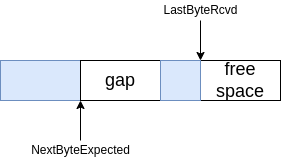
\includegraphics[width=200px]{images/6_Trasporto/free_space_calculation.png}
\end{figure}

\subsection{Controllo della congestione}
La congestione consiste nell' avere troppe sorgenti che inviano troppi dati troppo velocemente affinché la rete possa gestire tutto ciò.
Quando questo succede si ha perdita di pacchetti e delay lunghi perché le code si riempono.
Succede sui router intermedi che devono smistare il traffico.

A differenza del controllo di flusso, che riguarda sorgente e destinazione, il controllo della congestione riguarda i nodi intermedi della rete.

Possiamo avere due approcci risolutivi alla congestione:
\begin{itemize}
    \item Network-assisted: i router intermedi forniscono feedback agli host, possiamo segnalare singolarmente la congestione oppure dire esplicitamente a quale rateo inviare i pacchetti
    
    \item End-to-end: niente feedback dalla rete, si inferisce la congestione quando si hanno rallentamenti e perdita di pacchetti.
    Questo approccio conservativo è utilizzato dal TCP.
\end{itemize}


\subsubsection{Congestion control network assisted in ATM}
Il protocollo ATM mette a disposizione una classe di servizio con garanzia del troughput minimo detta ABR (available bit rate), questa classe di servizio deve implementare un meccanismo di controllo della congestione affinché possa garantire la banda minima.

Uno dei meccanismi che si possono utilizzare a tale scopo è RM cells: la sorgente tra i vari pacchetti di dati ne invia alcuni detti RM cells (resource management) con dei bit che possono essere settati dagli switch incontrati durante il percorso, questi bit sono:
\begin{itemize}
    \item NI bit: (no increase in rate) indica che c'è una leggera congestione e si dovrebbe evitare di aumentare il rate per non cadere nella congestione completa

    \item CI bit: (congestion indication) che indica che siamo effettivamente in una congestione e quindi sarebbe ottimale diminuire il rate
    
    \item byte ER: (explicit rate) il mittente inserisce all' interno il suo rateo corrente, ogni switch sul percorso può abbassarlo solamente in modo da indicare la velocità massima da tenere in caso di congestione
\end{itemize}
questi pacchetti inviati dal sender verso il receiver vengono poi rispediti dal ricevitore al sender con i bit modificati, possibilmente.
\begin{figure}[H]
    \centering
    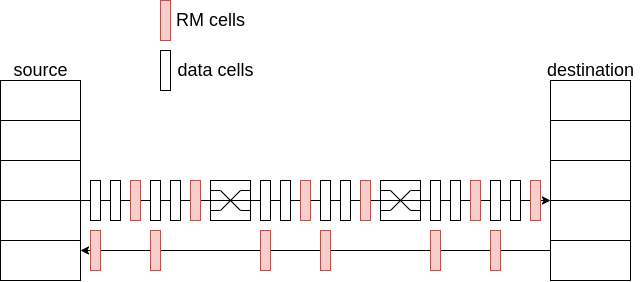
\includegraphics[width=330px]{images/6_Trasporto/ATM_ABR_congestion_control.png}
\end{figure}
Nelle celle di dati vi è anche il bit EFCI che viene settato ad 1 dagli switch congestionati, se la cella dato che precede una cella RM ha il bit EFCI settato il mittente setta il bit CI nelle celle RM che vengono rispedite indietro.


\subsubsection{Congestion control end-to-end in TCP}
L' obiettivo è far si che tutte le sorgenti possano trasmettere il più velocemente possibile senza che la rete si congestioni.

Per limitare il rate di trasmissione possiamo inviare meno byte nella stessa finestra di tempo, per fare questo abbassiamo il numero di segmenti non ackati nella pipeline ad un valore che chiameremo \verb{cwnd{ (congestion window) che rispetta:
$$ LastByteSent - LastByteAcked \leq cwnd $$

Questo valore in realtà viene scelto come il minimo tra la dimensione della congestion windows e la dimensione della receiver window, facendo così possiamo abbassare il rateo di pacchetti inviati.
Si noti che cwnd è dinamico e dipende dal livello di congestione della rete.

Per accorgersi di una congestione della rete il protocollo TCP si basa sugli ACK e sui segmenti perduti.
Se ho ottenuto ACK allora la rete non è congestionata e posso aumentare il rate, se ho dei segmenti persi invece assumo che la perdita sia dovuta alla congestione della rete e quindi abbasso il rateo di invio.
I paccheti persi sono sentiti tramite il time-out o 3 ACK duplicati.

L' idea di base dietro all' algoritmo è di fare \emph{probing} della bandwith:
\begin{itemize}
    \item quando ricevo degli ACK incremento il rateo di trasmissione (aumento di una quantità fissa)

    \item quando invece si hanno delle perdite si diminuisce il rate
\end{itemize}
L' andamento del rate è tipicamente a dente di sega perché segue questi aumenti e queste decrescite.

Dividiamo il protocollo in 3 fasi:
\begin{itemize}
    \item Slow start: aumentare linearmente la dimensione della finestra all' inizio è controproducente in quanto devo massimizzare il rateo il prima possibile, alla partenza abbiamo quindi come \verb{cwnd{ 1MSS (maximum segment size) e come rate MSS/RTT ed incrementiamo raddoppiando il rateo ad ogni ACK finché non superiamo un particolare threshold o non otteniamo una perdita di pacchetti.
    Una volta superato la threshold si va in fase congestion avoidance.
    
    Di default il threshold è 64Kbyte.

    \item Congestion avoidance: si incrementa linearmente cwnd ad ogni ACK.
    Quando si hanno 3 ACK duplicati modifichiamo:
    $$ threshold = \frac{cwnd}{2} $$
    $$ cwnd = \frac{cwnd}{2} + 3 \cdot MSS $$
    e si va in fast recovery.

    Quando si ha un timeout invece:
    $$ threshold = \frac{cwnd}{2} $$
    $$ cwnd = 1 $$
    e si torna in slow start.

    \item Fast recovery: 
    
\end{itemize}
\begin{figure}[H]
    \centering
    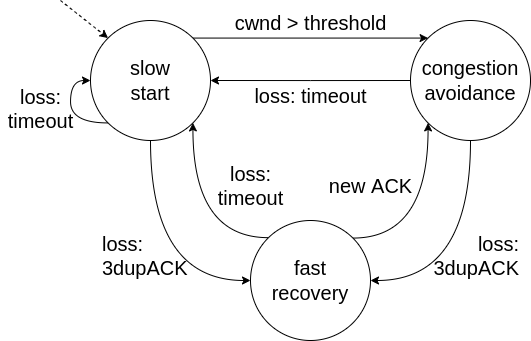
\includegraphics[width=250px]{images/6_Trasporto/TCP_congestion_control_FSM.png}
\end{figure}

Si noti che il TCP assume che qualsiasi packet loss sia dovuto alla congestione, questa assunzione non è vera nei casi in cui si usino dei link con perdite come i link wireless o le reti con nodi mobili.
Questo purtroppo porta ad abbassare il rateo anche quando non sarebbe strettamente necessario, è quindi consigliato implementare delle notifiche esplicite sulla congestione.

Il protocollo TCP è fair quindi se $K$ sessioni TCP condividono lo stesso bottleneck $R$ allora ogni sessione finirà ad avere rateo medio di $\frac{R}{K}$.
Vediamo una simulazione:
\begin{figure}[H]
    \centering
    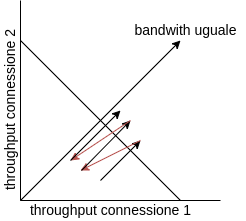
\includegraphics[width=200px]{images/6_Trasporto/TCP_fairness.png}
\end{figure}
Inizialmente si parte da uno scompenso tra le due connessioni, entrambe crescono linearmente perché in fase di congestion avoidance, appena la somma dei throughput supera la capacità del canale si avranno delle perdite di pacchetti o ACK triplicati quindi il protocollo vedrà questi eventi come una congestione e dimezzeranno il throughput, eseguendo questa procedura abbastanza volte si finisce a convergere sulla linea di bandwith uguale.



